% Authors: Greg Westphal and Kathryn Huff
\documentclass[border=10pt]{standalone}
\usepackage{tikz}
\usetikzlibrary{arrows.meta}
\tikzset{%
  >={Latex[width=2mm,length=2mm]},
  % Specifications for style of nodes:
            base/.style = {rectangle, rounded corners, draw=black,
                           minimum width=3cm, minimum height=1cm,
                           text centered, font=\sffamily},
       bluebox/.style = {base, fill=gray!15}, %blue!30
       redbox/.style = {base, fill=white!30}, %red
       greenbox/.style = {base, fill=white!30}, %green
       process/.style = {base, minimum width=2.5cm, fill=gray!30, %orange!15
                           font=\ttfamily},
}
% Drawing part, node distance is 1.5 cm and every node
% is prefilled with white background
\begin{document}
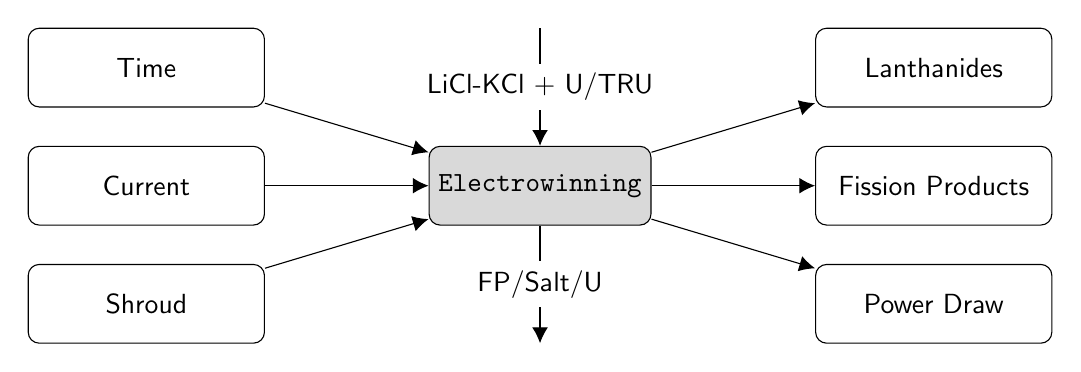
\begin{tikzpicture}[node distance=3cm,
    every node/.style={fill=white, font=\sffamily}, align=center]
  % Specification of nodes (position, etc.)
  
  \node (winning)			[process] {Electrowinning};
  \node (time)				[greenbox, left of=winning, xshift=-2cm, yshift=1.5cm] {Time};
  \node (current) 			[greenbox, left of=winning, xshift=-2cm] {Current};
  \node (shroud)			[greenbox, left of=winning, xshift=-2cm, yshift=-1.5cm] {Shroud};
  \node (cesium)			[redbox, right of=winning, xshift=2cm, yshift=1.5cm] {Lanthanides}; 
  \node (fission)			[redbox, right of=winning, xshift=2cm] {Fission Products};
  \node (power)				[redbox, right of=winning, xshift=2cm, yshift=-1.5cm] {Power Draw};
  %\node (fuel)				[process, below of=winning, xshift=-2cm] {Fuel \\ Fabrication};
  %\node (refining)			[process, below of=winning, yshift=1cm] {Electrorefining};
  
  \draw[->]					(winning)++(0,2) -- (winning) node[midway] {LiCl-KCl + U/TRU};
  \draw[->]					(winning) -- (fission);
  \draw[->] 				(winning) -- (cesium);
  \draw[->]					(winning) -- (power);
  \draw[->]					(time) -- (winning);
  \draw[->]					(current) -- (winning);
  \draw[->]					(shroud) -- (winning);
  %\draw[->]					(winning)++(-0.25,-0.5) -- ++(0,-1) -- ++(-1.75,0) node[midway] {U/TRU} -- (fuel);
  %\draw[->]					(winning) -- (refining) node[midway] {FP/Salt/U};
  \draw[->]					(winning) -- ++(0,-2) node[midway] {FP/Salt/U};

  \end{tikzpicture}
\end{document}